\usetikzlibrary{calc}
\begin{frame}{multiple APs, one network}
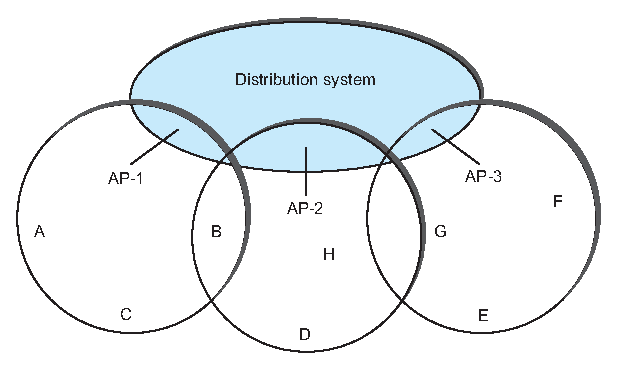
\includegraphics[width=\textwidth]{../multiaccess/cnsp-fig48}
\imagecredit{Computer Networks: A Systems Approach, figure 48}
\end{frame}

\begin{frame}{APs as switches}
    \begin{itemize}
    \item multiple APs can act as \textit{one network}
    \item example: nodes connected to different APs can send packets to each other by MAC address
    \vspace{.5cm}
    \item distribution system needs to share neighbor-table-like information
    \end{itemize}
\end{frame}

\begin{frame}{switching APs}
    \begin{itemize}
    \item nodes can switch APs\ldots
    \vspace{.5cm}
    \item check for new APs when signal strength too low
    \item periodically check for beacons + signal strength
    \vspace{.5cm}
    \item switching APs = same as joining network, but\ldots
        \begin{itemize}
        \item can keep IP address, etc.
        \item maybe optimizations to avoid redoing wifi security, etc.
        \end{itemize}
    \end{itemize}
\end{frame}

\begin{frame}{cellular networks}
    \begin{itemize}
    \item for wifi networks, feasible to track device locations centrally mostly
    \vspace{.5cm}
    \item need/have something more complex for cellular networks
    \end{itemize}
\end{frame}

\begin{frame}{a confusing picture}
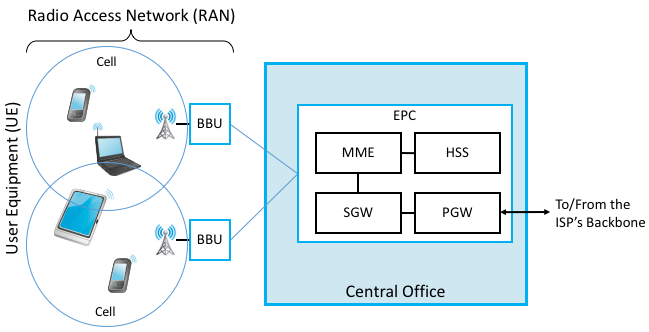
\includegraphics[width=\textwidth]{../multiaccess/sysapp-fig53}
\end{frame}

\begin{frame}{cellular mobility model}
    \begin{itemize}
    \item cellular networks: base stations don't know how to route to each end-host in whole cell network
    \vspace{.5cm}
    \item cell phone (UE) $\rightarrow$ base station (BBU) $\rightarrow$ service gateway (SGW) $\rightarrow$ PDN gateway (PGW)
    \vspace{.5cm}
    \item central `mobility management entity' (MME) sets up `tunnels' for steps above
        \begin{itemize}
        \item coordinates with home subscriber server (HSS)
        \item base stations don't track full routing information
        \end{itemize}
    \item PDN gateway stays stable so IP address can stay the same
        \begin{itemize}
        \item PDN gateway = gateway to actual Internet
        \end{itemize}
    \item in `roaming' situation:
        \begin{itemize}
        \item service gateway run by network you're connected to
        \item PDN gateway run by `home' network
        \end{itemize}
    \end{itemize}
\end{frame}

